\lecture{2}{27. August 2025}{Basic equations of fluid statics and buoyancy, surface tension}

\section{Fluid Statics}

\subsection{The basic equations of fluid statics}
Consider a differential fluid element of mass $\mathrm{d}m = \rho \, \mathrm{d}V$ with sides $\mathrm{d}x $, $\mathrm{d}y$, and $\mathrm{d}z$ as shown on \textbf{\autoref{fig:f3_1}}. The fluid element is stationary relative to the coordinate system shown.

\begin{figure} [htpb]
  \centering
  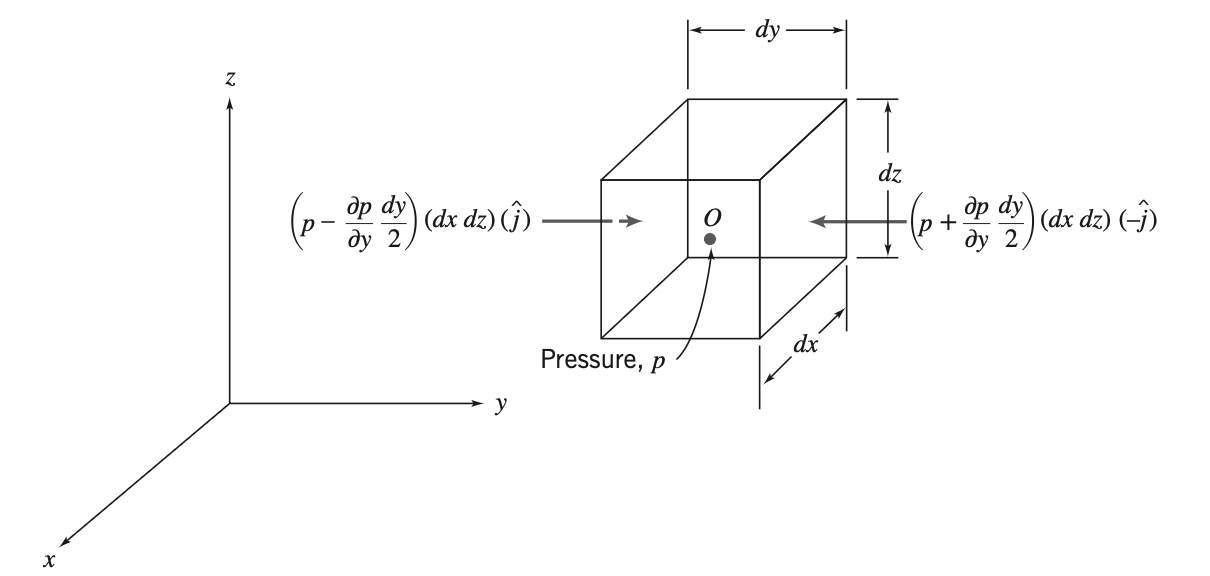
\includegraphics[width=0.5\linewidth]{./figures/f3_1.png}
  \caption{Differential fluid element with pressure forces shown in the $y$-direction}
  \label{fig:f3_1}
\end{figure}

It has previously been mentioned that only \textit{body forces} and \textit{surface forces} may be applied to a fluid. In this course the body forces caused by electric or magnetic fields is assumed negligible and only the gravitational force must therefore be accounted for.

For the differential fluid element the (gravitational) body force is:
\[ 
  \mathrm{d}\textbf{F}_B = \textbf{g} \, \mathrm{d}m = \textbf{g} \rho \, \mathrm{d}V
.\]
where $\textbf{g}$ denotes the local gravity vector, $\rho$ is the density and $\mathrm{d}V$ is the volume of the fluid element. This can also be expressed as:
\[ 
\mathrm{d} \textbf{F}_B = \rho \textbf{g} \, \mathrm{d}x \, \mathrm{d}y \, \mathrm{d}z
.\]
Per definition there can be no shear stresses in a static fluid, so the only surface force is that due to pressure, which is a scalar field, $p = p(x,y,z)$. The net pressure force can be found by summing the forces on each of the six faces of the fluid element. The pressure at the center $O$ is denoted $p$. The pressure at each face of the element will be found using a Taylor series expansion of the pressure about point O. The pressure on the left side of the fluid element is:
\[ 
p_L = p + \frac{\partial p}{\partial y} \left( y_L - y \right) = p + \frac{\partial p}{\partial y} \left( - \frac{\mathrm{d}y}{2} \right) = p - \frac{\partial p}{\partial y} \frac{\mathrm{d}y}{2}
.\]
Terms of higher order are omitted as they will vanish at a later step anyways. Similarly, the pressure on the right face of the differential element is:
\[ 
p_R = p \frac{\partial p}{\partial y} \left( y_R - y \right) = p + \frac{\partial p}{\partial y} \frac{\mathrm{d}y}{2}
.\]
The pressure \textit{forces} produced by this pressure is shown on \textbf{\autoref{fig:f3_1}}. These consist of three factors. Namely the magnitude of the pressure, the area of the face and a unit vector to indicate direction. A positive pressure here is defined as a compressive pressure on the differential element. The pressure forces in the other directions can be obtained in the same way giving:
\begin{align*}
  \mathrm{d}\textbf{F}_S &= \left( p - \frac{\partial p}{\partial x} \frac{\mathrm{d}x}{2} \right) \left( \mathrm{d}y \, \mathrm{d}z \right) \left( \hat{\textbf{i}} \right) + \left( p + \frac{\partial p}{\partial x} \frac{\mathrm{d}x}{2} \right) \left( \mathrm{d}y \, \mathrm{d}z \right) \left( - \hat{\textbf{i}} \right) \\
                         &+ \left( p - \frac{\partial p}{\partial y} \frac{\mathrm{d}y}{2} \right) \left(\mathrm{d}x \, \mathrm{d}z \right) \left( \hat{\textbf{j}} \right) + \left( p + \frac{\partial p}{\partial y} \frac{\mathrm{d}y}{2} \right) \left( \mathrm{d}x \, \mathrm{d}z \right) \left( - \hat{\textbf{j}} \right) \\
                         &+ \left( p - \frac{\partial p}{\partial z} \frac{\mathrm{d}z}{2} \right) \left( \mathrm{d}x \, \mathrm{d}y  \right) \left( \hat{\textbf{k}} \right) + \left( p + \frac{\partial p}{\partial z} \frac{\mathrm{d}z}{2} \right) \left( \mathrm{d}x \, \mathrm{d}y  \right) \left( - \hat{\textbf{k}} \right)
.\end{align*}
Simplifying this, we obtain
\[ 
  \mathrm{d}\textbf{F}_S = - \left( \frac{\partial p}{\partial x} \hat{\textbf{i}} + \frac{\partial p}{\partial y} \hat{\textbf{j}} + \frac{\partial p}{\partial z} \hat{\textbf{k}} \right) \, \mathrm{d}x \, \mathrm{d}y \, \mathrm{d}z
.\]
We can now recognize the term in the parentheses as the gradient of the pressure which may be written as either $\mathrm{grad} p$ or $\nabla p$. This is:
\[ 
  \mathrm{grad} p \equiv \nabla p \equiv \left( \hat{\textbf{i}} \frac{\partial p}{\partial x} + \hat{\textbf{j}} \frac{\partial p}{\partial y} + \hat{\textbf{k}} \frac{\partial p}{\partial z}  \right) \equiv \left( \hat{\textbf{i}} \frac{\partial }{\partial x} + \hat{\textbf{j}}\frac{\partial }{\partial y} + \hat{\textbf{k}} \frac{\partial }{\partial z} \right) p
.\]
Using this notation we can rewrite the expression as:
\[ 
\mathrm{d}\textbf{F}_S = - \mathrm{grad} p(\mathrm{d}x \, \mathrm{d}y \, \mathrm{d}z) = - \nabla p \, \mathrm{d}x \, \mathrm{d}y \, \mathrm{d}z
.\]
Note that the pressure magnitude is not relevant when computing the net pressure force -- instead only the rate of change of pressure with distance, the pressure gradient, is needed. 

We can now combine the expressions for the surface and body forces on the fluid element.
\[ 
\mathrm{d}\textbf{F} = \mathrm{d}\textbf{F}_S + \mathrm{d}\textbf{F}_B = \left( - \nabla p + \rho \textbf{g} \right) \, \mathrm{d}x \, \mathrm{d}y \, \mathrm{d}z = \left( - \nabla p + \rho \textbf{g} \right) \mathrm{d}V
\]
which can also be stated as the force acting per unit volume as
\[ 
\frac{\mathrm{d}\textbf{F}}{\mathrm{d}V} = - \nabla p + \rho \textbf{g} 
.\]
Applying Newton's second law to a static fluid particle gives
\[ 
\textbf{F} = \textbf{a} \, \mathrm{d}m = \textbf{0} \, \mathrm{d}m = \textbf{0}
.\]
Thus
\[ 
\frac{\mathrm{d}\textbf{F}}{\mathrm{d}V} = \rho \textbf{a} = \textbf{0} 
.\]
Combining these two gives:
\[ 
- \nabla  p + \rho \textbf{g} = \textbf{0}
.\]
This can be stated in words as the sum of the net pressure force per unit volume at a point and the body force per unit volume at a point is zero. As this is a three-dimensional vector equation it is comprised of three individual equations that must each be satisfied individually.
\begin{align*}
  - \frac{\partial p}{\partial x} + \rho g_x &= 0 \\
  - \frac{\partial p}{\partial y} + \rho g_y &= 0 \\
  - \frac{\partial p}{\partial z} + \rho g_z &= 0
.\end{align*}
It is now convenient to choose a coordinate system such that the gravity vector is aligned with one of the axes. If we place the coordinate system ``normally'' we would get $g_x = 0$, $g_y = 0$, and $g_z = -g$. The component equations then become
\begin{align*}
  \frac{\partial p}{\partial x} &= 0 \\
  \frac{\partial p}{\partial y} &= 0 \\
  \frac{\partial p}{\partial z} &= -\rho g
.\end{align*}
This means that the pressure depends on one variable only and the total derivative may therefore be employed instead of the partial as
\[ 
\frac{\partial p}{\partial z} = - \rho g \equiv -\gamma
.\]
This is the basic pressure-height relation of fluid statics. 

\subsection{Pressure variation in a static fluid}

\subsubsection{Incompressible fluids}
For an incompressible fluid $\rho = \mathrm{constant}$. If we assume the gravity to be constant with elevation then we get
\[ 
\frac{\partial p}{\partial z} = - \rho g = \mathrm{constant}
.\]
Now we can easily integrate this as
\[
  \int_{p_0}^{p} \, \mathrm{d}p = - \int_{z_0}^{z} \rho g \, \mathrm{d}z \\
.\]
The height difference is defined as $h = z_0 - z$ and thus we upon integration obtain
\[ 
p - p_0 = \Delta p = \rho gh
.\]

To find the pressure difference $\Delta p$ between two points separated by a series of fluid, we can compute the change in pressure as
\[ 
\Delta p = g \sum_{i} \rho_i h_i 
.\]

\subsubsection{Gases}
Pressure variation in a compressible fluid must be found by integration of the previous result. First, however, an expression for the density as a function of either $p$ or $z$ must be found. To do this we employ the ideal gas law:
\[ 
p = \rho R T
.\]
Here the temperature $T$ is introduced as an additional variable. In the U.S. Standard Atmosphere, the temperature decreases linearly with altitude up to an elevation of \qty{11,0}{km}. Therefore the temperature can be expressed as:
\[ 
T = T_0 - mz
.\]
We therefore get
\[ 
\mathrm{d}p = - \rho g \, \mathrm{d}z = - \frac{pg}{RT} \, \mathrm{d}z = - \frac{pg}{R \left( T_0 - mz \right)} \, \mathrm{d}z
.\]
By separation of variables we obtain:
\[ 
\int_{p_0}^{p} \frac{\mathrm{d}p}{p}= - \int_{0}^{z} \frac{g \, \mathrm{d}z}{R \left( T_0 - mz \right)}
.\]
Which gives
\[ 
\ln \frac{p}{p_0} = \frac{g}{mR} \ln \left(  \frac{T_0 - mz}{T_0} \right) = \frac{g}{mR} \ln \left( 1 - \frac{mz}{T_0} \right)
.\]
Which can be solved for $p$ as
\[ 
p = p_0 \left( 1 - \frac{mz}{T_0} \right)^{\frac{g}{mR}} = p_0 \left( \frac{T}{T_0} \right)^{\frac{g}{mR}}
.\]

\subsection{Buoyancy}
Any object submerged in a liquid will experience a vertical force acting on it due to liquid pressure -- this is termed \textit{buoyancy}. Consider the object on \textbf{\autoref{fig:f3_9}} which is split into cylindrical volume elements.

\begin{figure} [ht]
  \centering
  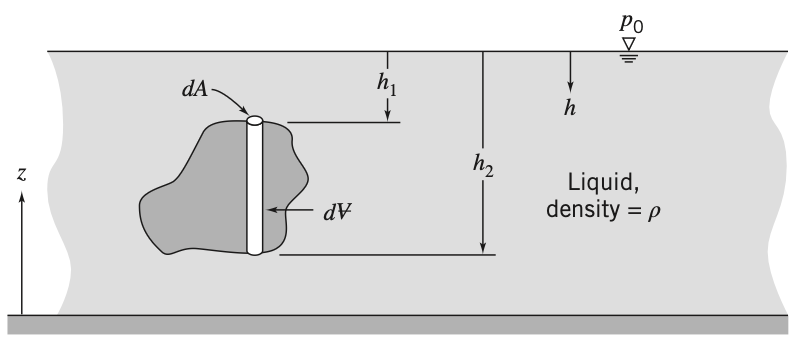
\includegraphics[width=0.5\linewidth]{./figures/f3_9.png}
  \caption{Immersed body in a static liquid.}
  \label{fig:f3_9}
\end{figure}

We have previously derived an equation for the pressure $p$ at depth $h$ in a liquid:
\[ 
p = p_0 + \rho gh
.\]
The net vertical force on the element is thus
\[ 
\mathrm{d}F_z = \left( p_0 + \rho gh_2 \right) \, \mathrm{d}A - \left( p_0 + \rho gh_1 \right) \, \mathrm{d}A = \rho g \left( h_2 - h_1 \right) \, \mathrm{d}A
.\]
As $\left( h_2 -  h_1 \right) \, \mathrm{d}A = \mathrm{d}V$ we get
\[ 
F_z = \int \, \mathrm{d}F_z = \int_{V} \rho g \, \mathrm{d}V = \rho g V
.\]
I.e. for a submerged body, the buoyancy force is equal to the weight of the displaced fluid. 
